\chapter{Funktioner}
\section{Funktioner och funktionsgrafer}
En funktion beskriver sambandet mellan in- och ut-data och kan bidra till ökad förståelse av hur olika processer hänger ihop.
%nästa mening är inte essentiell för kursen, kan antagligen raderas
Klassisk machine learning handlar mycket om att just hitta bra funktioner för att relatera in- och ut-data (supervised learning).

I envariabelanalys studeras funktioner som relaterar ett tal till ett annat.
Kan tänkas som en "regel" $f$ som \underline{avbildar} ett givet tal $x$ till ett annat tal $y$.

Alla de värdena som är tillåtna att mata in i $f$ kallas för funktionens \underline{definitionsmängd} och betecknas $D(f)$.
Mängden av alla $y$-värden som funktionen kan leverera kallas för \underline{värdemängden} och skrivs $R(f)$ (range).

\paragraph{Ex} Funktionen $f(x)=\frac{1}{x^2-1}$ har $D(f)=(-\infty,-1)\cup(-1,1)\cup(1,\infty)$.

\paragraph{} En funktionsgraf (eller bara en graf) givet en funktion $f$ utgörs av alla punkter $(x,y)=(x,f(x))$.
Några viktiga concept:
\begin{itemize}
    \item En funktion sägs vara \underline{jämn} om $f(-x)=f(x)$ då $(x\in D(f))$.\\
          Betyder att $f$ är symmetrisk m.a.p. y-axeln.
    \item En funktion sägs vara \underline{udda} om $f(-x)=-f(x)$.\\
          Betyder att $f$ är \underline{antispegelsymmetrisk} m.a.p. y-axeln.
    \item En funktion är \underline{injektiv} om det för varje par $x_1,x_2\in D(f)$ gäller att om $f(x_1)=f(x_2)$ så är $x_1=x_2$.
    \item En funktion $f$ som avbildar en mängd tal $\bm{x}$ på en annan mängd $\bm{y}$, dvs $f:\bm{x}\rightarrow\bm{y}$ sägs vara \underline{surjektiv} om $\bm{y}=R(f)$.
\end{itemize}

\section{Kompositioner}
En vanlig konstruktion är att kombinera två separata funktioner till en ny genom \underline{komposition}.
Kan göras på två sätt:
\begin{enumerate}
    \item $f\circ g(x):=f(g(x))$
    \item $g\circ f(x):=g(f(x))$
\end{enumerate}
Notera att $f\circ g\neq g\circ f$ i allmänhet!

\chapter{Polynom och rationella funktioner}
Ett polynom är en funktion som kan skrivas som:
$P(x)=a_1\cdot x^n+a_{n-1}\cdot x^{n-1}+...+ax+a_0$ där $a_n,... ,a_0\in\mathbb{R}$ kallas för polynomets \underline{koefficienter} och talet $n$ (positivt heltal) kallas för polynomets \underline{grad}.
En rationell funktion $R(x)$ är en funktion som kan skrivas som en kvot på två polynom $P(x)$ och $Q(x)$, dvs $R(x)=\frac{P(x)}{Q(x)}$.
Definitionsmängden $D(R)$ begränsas enbart av nollställena till $Q(x)$, dvs. $D(R)=\mathbb{R}\setminus \{x\in\mathbb{R}:Q(x)=0\}$.

\section{Polynomdivision}
Rationella tal kan alltid skrivas som en heltalsdel + rest:\\
$\frac{29}{6}=\frac{4*6+5}{6}=\frac{4*6}{6}+\frac{5}{6}=4+\frac{5}{6}$\\
Motsv. funkar även för rationella funktioner  och metoden för att hita "heltalsdelen" och "resten" kalla \underline{polynomdivison}.

\paragraph{Ex (P6.18)} Uttryck $\frac{x^4+x^2}{x^3+x^2+1}$ som summan av ett polynom och en rationell funktion.
\subparagraph{Lösning}~\\
\begin{wrapfigure}{l}{0.4\textwidth}
    \vspace{-15pt}
    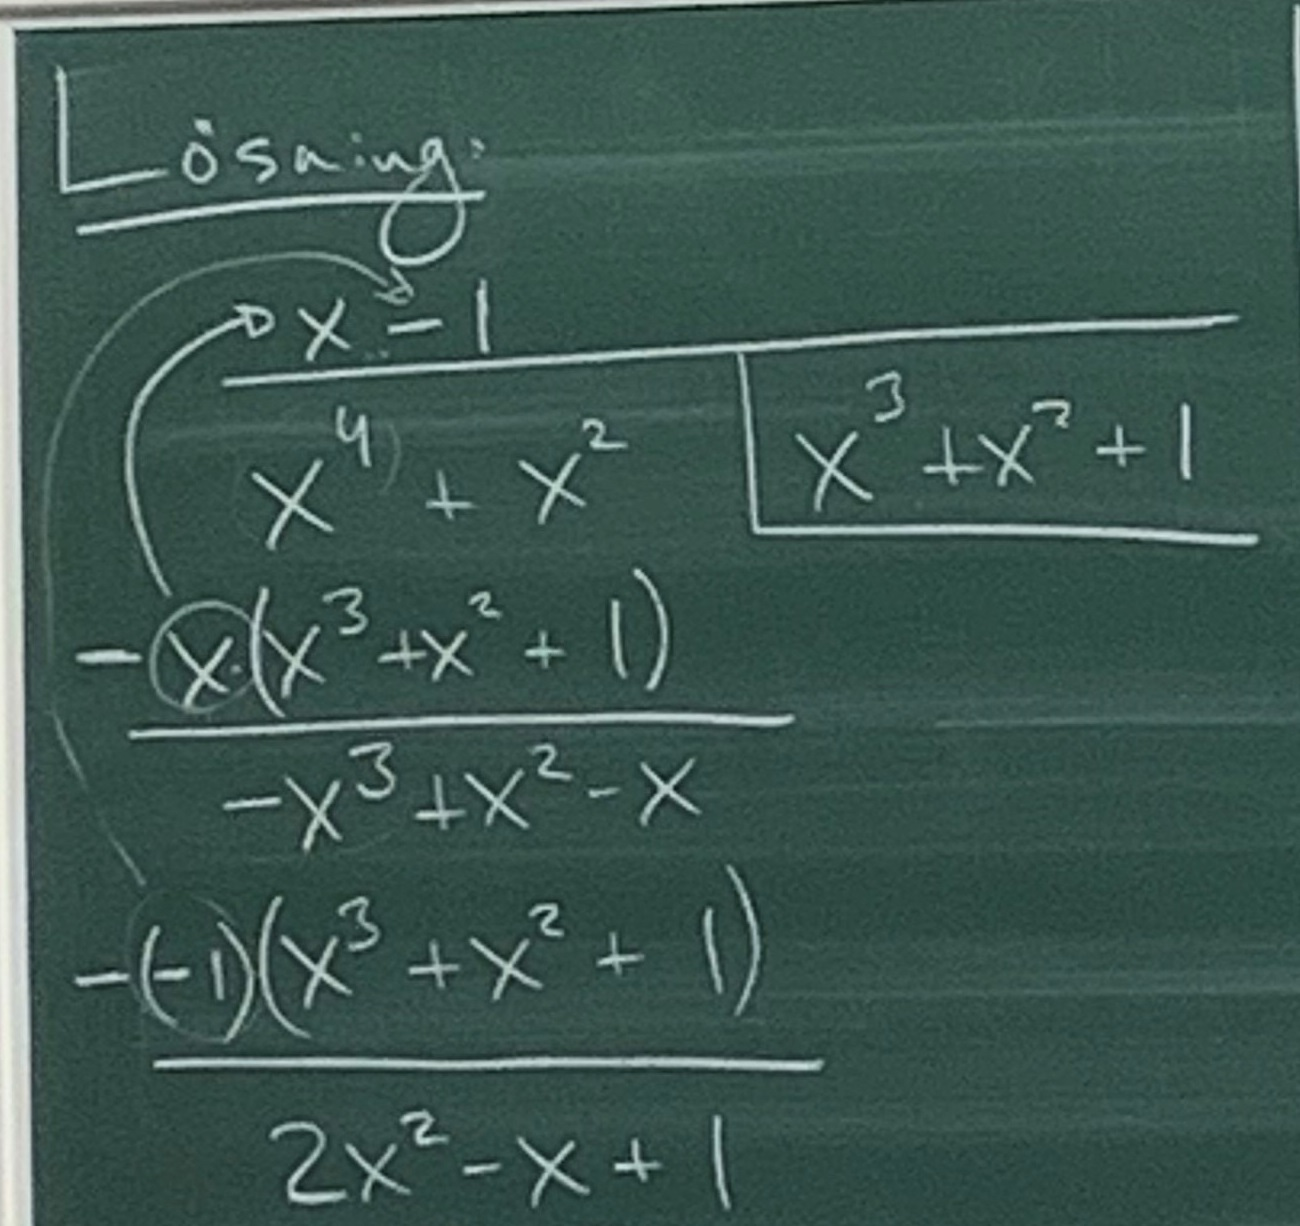
\includegraphics[scale=0.1]{lessons/lesson02/imgs/img01.jpg}\\
\end{wrapfigure}
Eftersom polynomet $2x^2-x+1$ har lägre grad än nämnaren $x^3+x^2+1$ tar divisionsalgo. slut.
Vi har fått att $\frac{x^4+x^2}{x^3+x^2+1}=(x-1)+\frac{2x^2-x+1}{x^3+x^2+1}\Box$.
\clearpage
\paragraph{} Enligt \underline{Aritmetikens fundamentalsats} så kan \underline{alla} positiva heltal alltid skrivas som en unik faktorisering av \underline{primtal}, t.ex $120=2^3\cdot 3\cdot 5$.
Liknande resultat finns för polynom! Algebrans fundementsats säger att varje polynom av grad $n$ har exakt $n$ st. nollställen (ev. komplexa och räknade med multiplicitet).
Vidare gäller också \underline{faktorsatsen}:
\paragraph{Sats} Talet $r$ är en \underline{rot} (dvs ett nollställe) till ett polynom $P$ av grad minst $1$ \underline{om och endast om} $(x-r)$ är en faktor av $P(x)$.
\\\\
Eftersom alla polynom $P$ av grad $\geq 1$ har precis $n$ st. nollställen säg $r_1,...,r_n$ kan man \underline{alltid} faktorisera ett polynom som $P(x)=(x-r_1)\cdot(x-r_2)\cdot ... \cdot(x-r_n)$.

\chapter{Grundläggande trigonometri}
De trigonometriska frunktionererna $\cos\theta$ och $\sin\theta$ def. som $x$- respektive y-koordinaten på den punkt på \underline{enhetscirkeln} som motsvaras av vinkeln $\theta$.
\begin{figure}[h!]
    \centering
    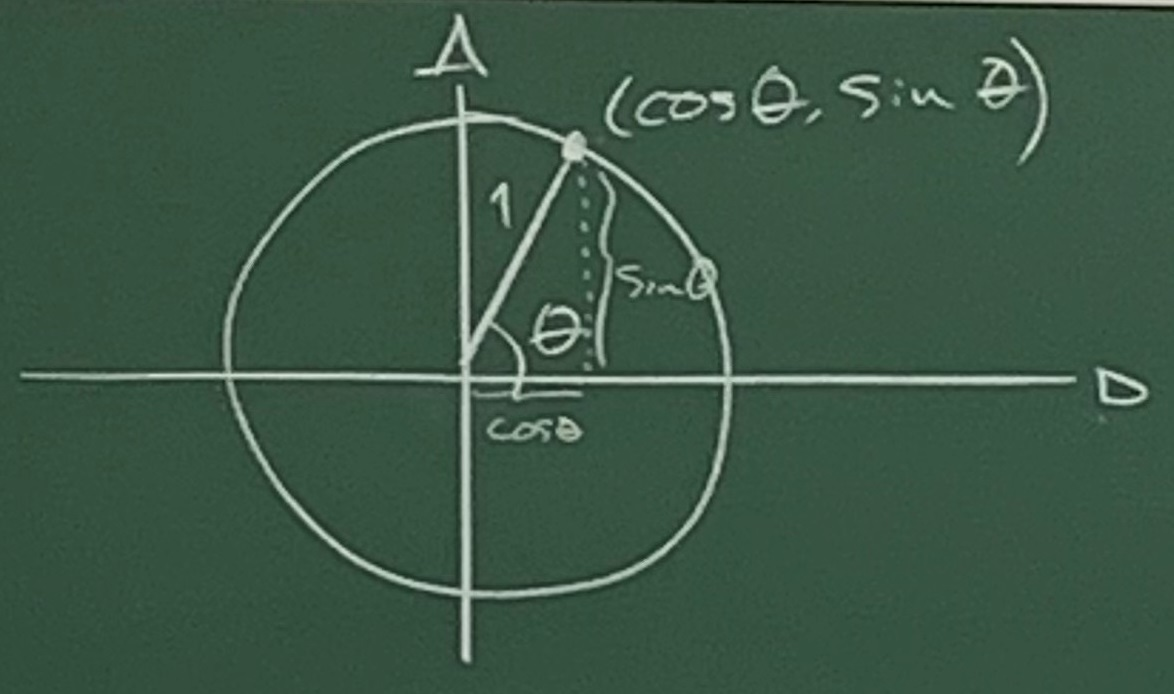
\includegraphics[scale=0.2]{lessons/lesson02/imgs/img02.jpg}
\end{figure}
Pythagoras sats ger omedelbart att $\cos^2\theta+\sin\theta=1$, även kallat trigonometriska ettan.
Vinkeln $\theta$ mäts oftast i radianer men kan också mätas i geader.
Det gäller att $\pi$ radianer motsvarar $180^\circ$ grader.

\paragraph{}Utifrån $\sin$ och $\cos$ definieras vidare funktionen tangens som $tan\theta:=\frac{\sin\theta}{\cos\theta}$.
Två trigonometriska samband som är viktiga är sinus- och cosinus-satsen:
%infoga bild 3
\begin{figure}[h!]
    \centering
    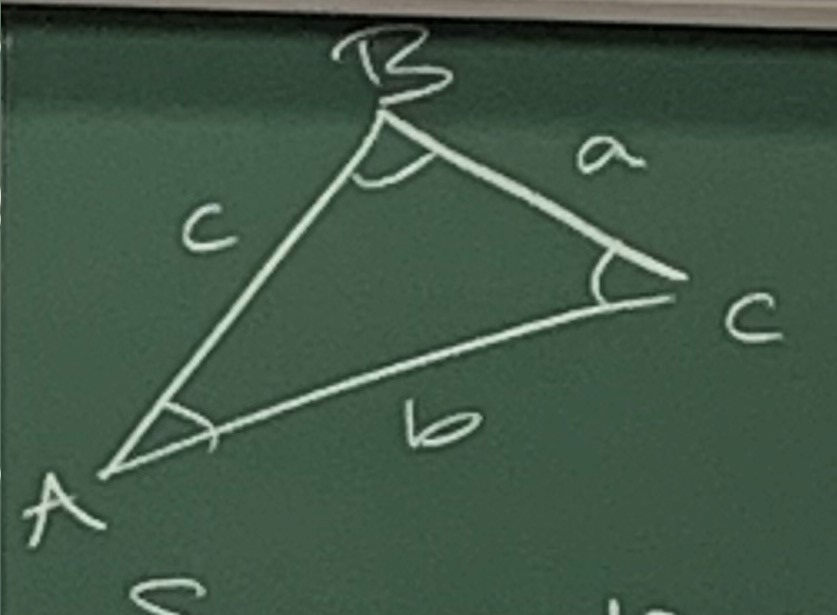
\includegraphics[scale=0.1]{lessons/lesson02/imgs/img03.jpg}
\end{figure}
\subparagraph{Sinussatsen} $\frac{\sin A}{a}=\frac{\sin B}{b}=\frac{\sin C}{c}$
\subparagraph{Cosinussatsen} $a^2=b^2+c^2-2b\cos A$

\paragraph{Ex (P6.53)} Visa att arean på en godtycklig triangel $ABC$ kan beräknas som $\frac{1}{2}bc\cdot\sin A=\frac{1}{2}ab\cdot\sin C=\frac{1}{2}ac\cdot\sin B$.
\subparagraph{Lösning}
Area$=\frac{x_z\cdot y}{2}+\frac{x_2\cdot y}{2}=\frac{x_1\cdot y + x_2\cdot y}{2}$.
Men $\sin A=\frac{y}{c}\Rightarrow y=c\cdot\sin A \Rightarrow Area=\frac{x_1\cdot c\sin A+x_2c\sin A}{2}=\frac{(x_1+x_2)\cdot c\cdot\sin A}{2}=\{x_1+x_2=b\}=\frac{1}{2}bc\sin A$.
De andra formulerna följer analogt. $\Box$
\begin{figure}[h!]
    \centering
    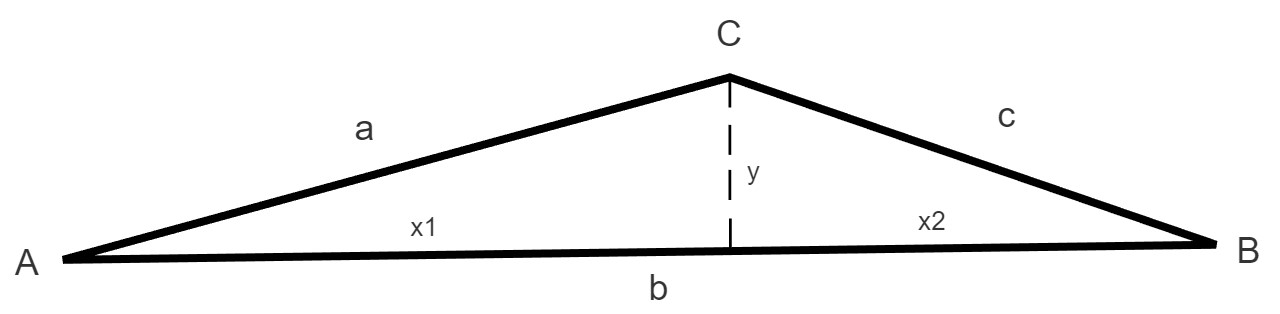
\includegraphics[scale=0.2]{lessons/lesson02/imgs/img04.jpg}
\end{figure}